\documentclass[a4paper, 10pt]{article}
\usepackage{pgfplots} % Used for plotting functions

\pgfplotsset{compat=1.18} % Add this line to set the compatibility version


\usepackage[margin = 1in]{geometry} % for spacing around
\usepackage{graphicx} % for including images in your pdfs
\usepackage{xcolor} % for including colors in your pdf
\usepackage{soul} % for text decoration
\usepackage[utf8]{inputenc} % for encoded text
\usepackage[T1]{fontenc}
\usepackage{setspace} % for setting different line spacings between paragrafs.
\usepackage{enumerate} % for letting us get more detailed enumerate lists
\usepackage{multirow} % to let us combine more rows together
\usepackage{colortbl} % for decorating tables
\usepackage{amsmath} % used for representing more complicated math displays
\usepackage{supertabular}
\usepackage{longtable} % both of these packages are used to making really big tables
\usepackage{wrapfig} % allows us to wrap text around figures
\usepackage{fancyhdr} % for making fancy headers
%\usepackage{bibtex} % for making better bibliographies
\usepackage[pdftex]{hyperref} % for letting us make links
\usepackage{lscape} % Allows us to flip from portrait to landspace
\usepackage{tikz} % for high detailed drawing
\usepackage{multicol} % To put things side by side
\usepackage{rotating} % For rotating objects
% \usepackage{draftwatermark} % For adding watermarks
\usepackage{MnSymbol} % for using multiple symbols
\usepackage{mathtools} % Used for more math symbols
\usepackage{xfrac} % For more complciated fractions and to add derivitives
\usepackage{hyperref} % for hyper links
\usepackage{enumitem} % for better enum lists
\usepackage{tcolorbox} % for adding colored text boxes
\usepackage{bm} % Adding bold text to math inputs
\usepackage{pgfplots} % Used for plotting functions
\usepackage{booktabs} % For prettier tables
\usepackage{subcaption} % For subfigures
\usepackage{siunitx} % Add the siunitx package for number column alignment

% Setting up the default image path
\graphicspath{{../../global-assets/images/}}

% Implementing authro details
\title{Lab Report number I - Title of the lab report\\
	ENS203 - Electrical Circuits I}
\author{Emre Arapcic-Uevak\\220302289}
\date{}

% Setting up the fancy page style
\fancypagestyle{customStyle}{
	\lhead{} \chead{} \rhead{}
	\lfoot{} \cfoot{\thepage} \rfoot{}
	\renewcommand{\headrulewidth}{0pt}
	\renewcommand{\footrulewidth}{1pt}
}
\pagestyle{customStyle}

% Custom commands

\begin{document}
	\begin{titlepage}
		\begin{center}
			\vspace*{\stretch{1}} % Add vertical space before the title

			{\Large\bfseries Lab Report number 5 \\[0.5em] Wheatstone Bridge\par}
			\vspace{1cm} % Space between title and course title

			{\large ENS203 – Electrical Circuits I\par}
			\vspace{1cm} % Space between course title and your name/ID

			{\large Emre Arapcic-Uevak \\ 220302289\par}
			\vspace{1cm} % Space between your name/ID and assistant name

			{\large Afan Haznadarevic \\ 220302128\par}
			\vspace{.5cm} % Space between your name/ID and assistant name

			{\large Assistant: Adil Hasanbasic\par}
			\vspace{\stretch{2}} % Variable vertical space between assistant name and bottom
			
\includegraphics[width=0.5\textwidth]{Logo.png}
			\vspace{5mm}
			
			\textsc{\LARGE Internation University of Sarajevo}\\[1.5cm]
			\textsc{\Large ENS203 - Electrical Circuits I}\\[0.5cm]
			
			\rule{\linewidth}{0.5mm} \\[0.4cm]
			{ \huge \bfseries Lab Report number V - Wheatstone bridge}\\[0.4cm]
			\rule{\linewidth}{0.5mm} \\[1.5cm]
			
			\vfill
			
			% Bottom of the page
			{\large \today}
		\end{center}
	\end{titlepage}
	\pagebreak

	\tableofcontents
	\pagebreak
	
	\listoffigures
	\pagebreak

	\listoftables	
	\pagebreak 
	
	\section{Objective}
		\subsection{Wheatstone}
			\begin{figure}[h!]
				\centering
				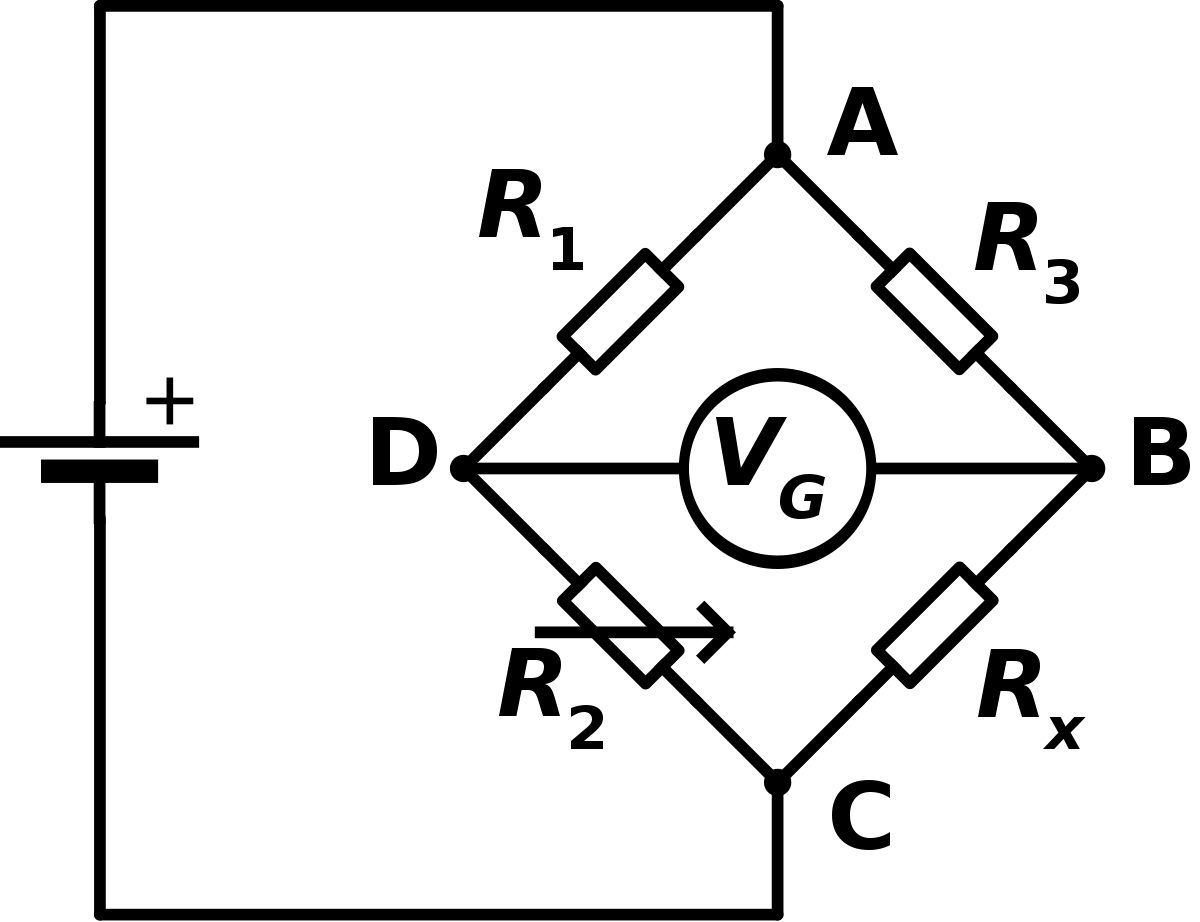
\includegraphics[width=0.5\textwidth]{./images/WheatstoneBridge.png}
				\caption{Wheatstone Bridge}
				\label{fig:wheatstone}
			\end{figure}

			The wheatstone bridge is a circuit that is used to measure an unknown resistance. 
			The circuit consists of four resistors, two of which are known, 1 variable resistor, and 1 unknown resistor.
			The circuit is balanced when the voltage between the two nodes is zero. 
			When the circuit is balanced, the ratio of the two known resistors is
			equal to the ratio of the two unknown resistors, or in other words 
			\begin{equation}
				\frac{R_1}{R_2} = \frac{R_3}{R_x}
			\end{equation}
			then we know that $V_D = V_B$, so the potential difference between the two nodes, $V_{DB}$, is zero.

			In today's lab, we will be using the wheatstone bridge and a multimeter to see when the bridge
			is balanced.

		\subsection{Apparatus}
			\begin{itemize}
				\item Multimeter
				\item Potenciometer
				\item Resistors
				\item DC Power Supply
				\item Breadboard
			\end{itemize}

			\pagebreak
			\subsubsection{DC Power Supply}
				Used to provide a constant voltage
				\begin{figure}[h!]
					\centering
					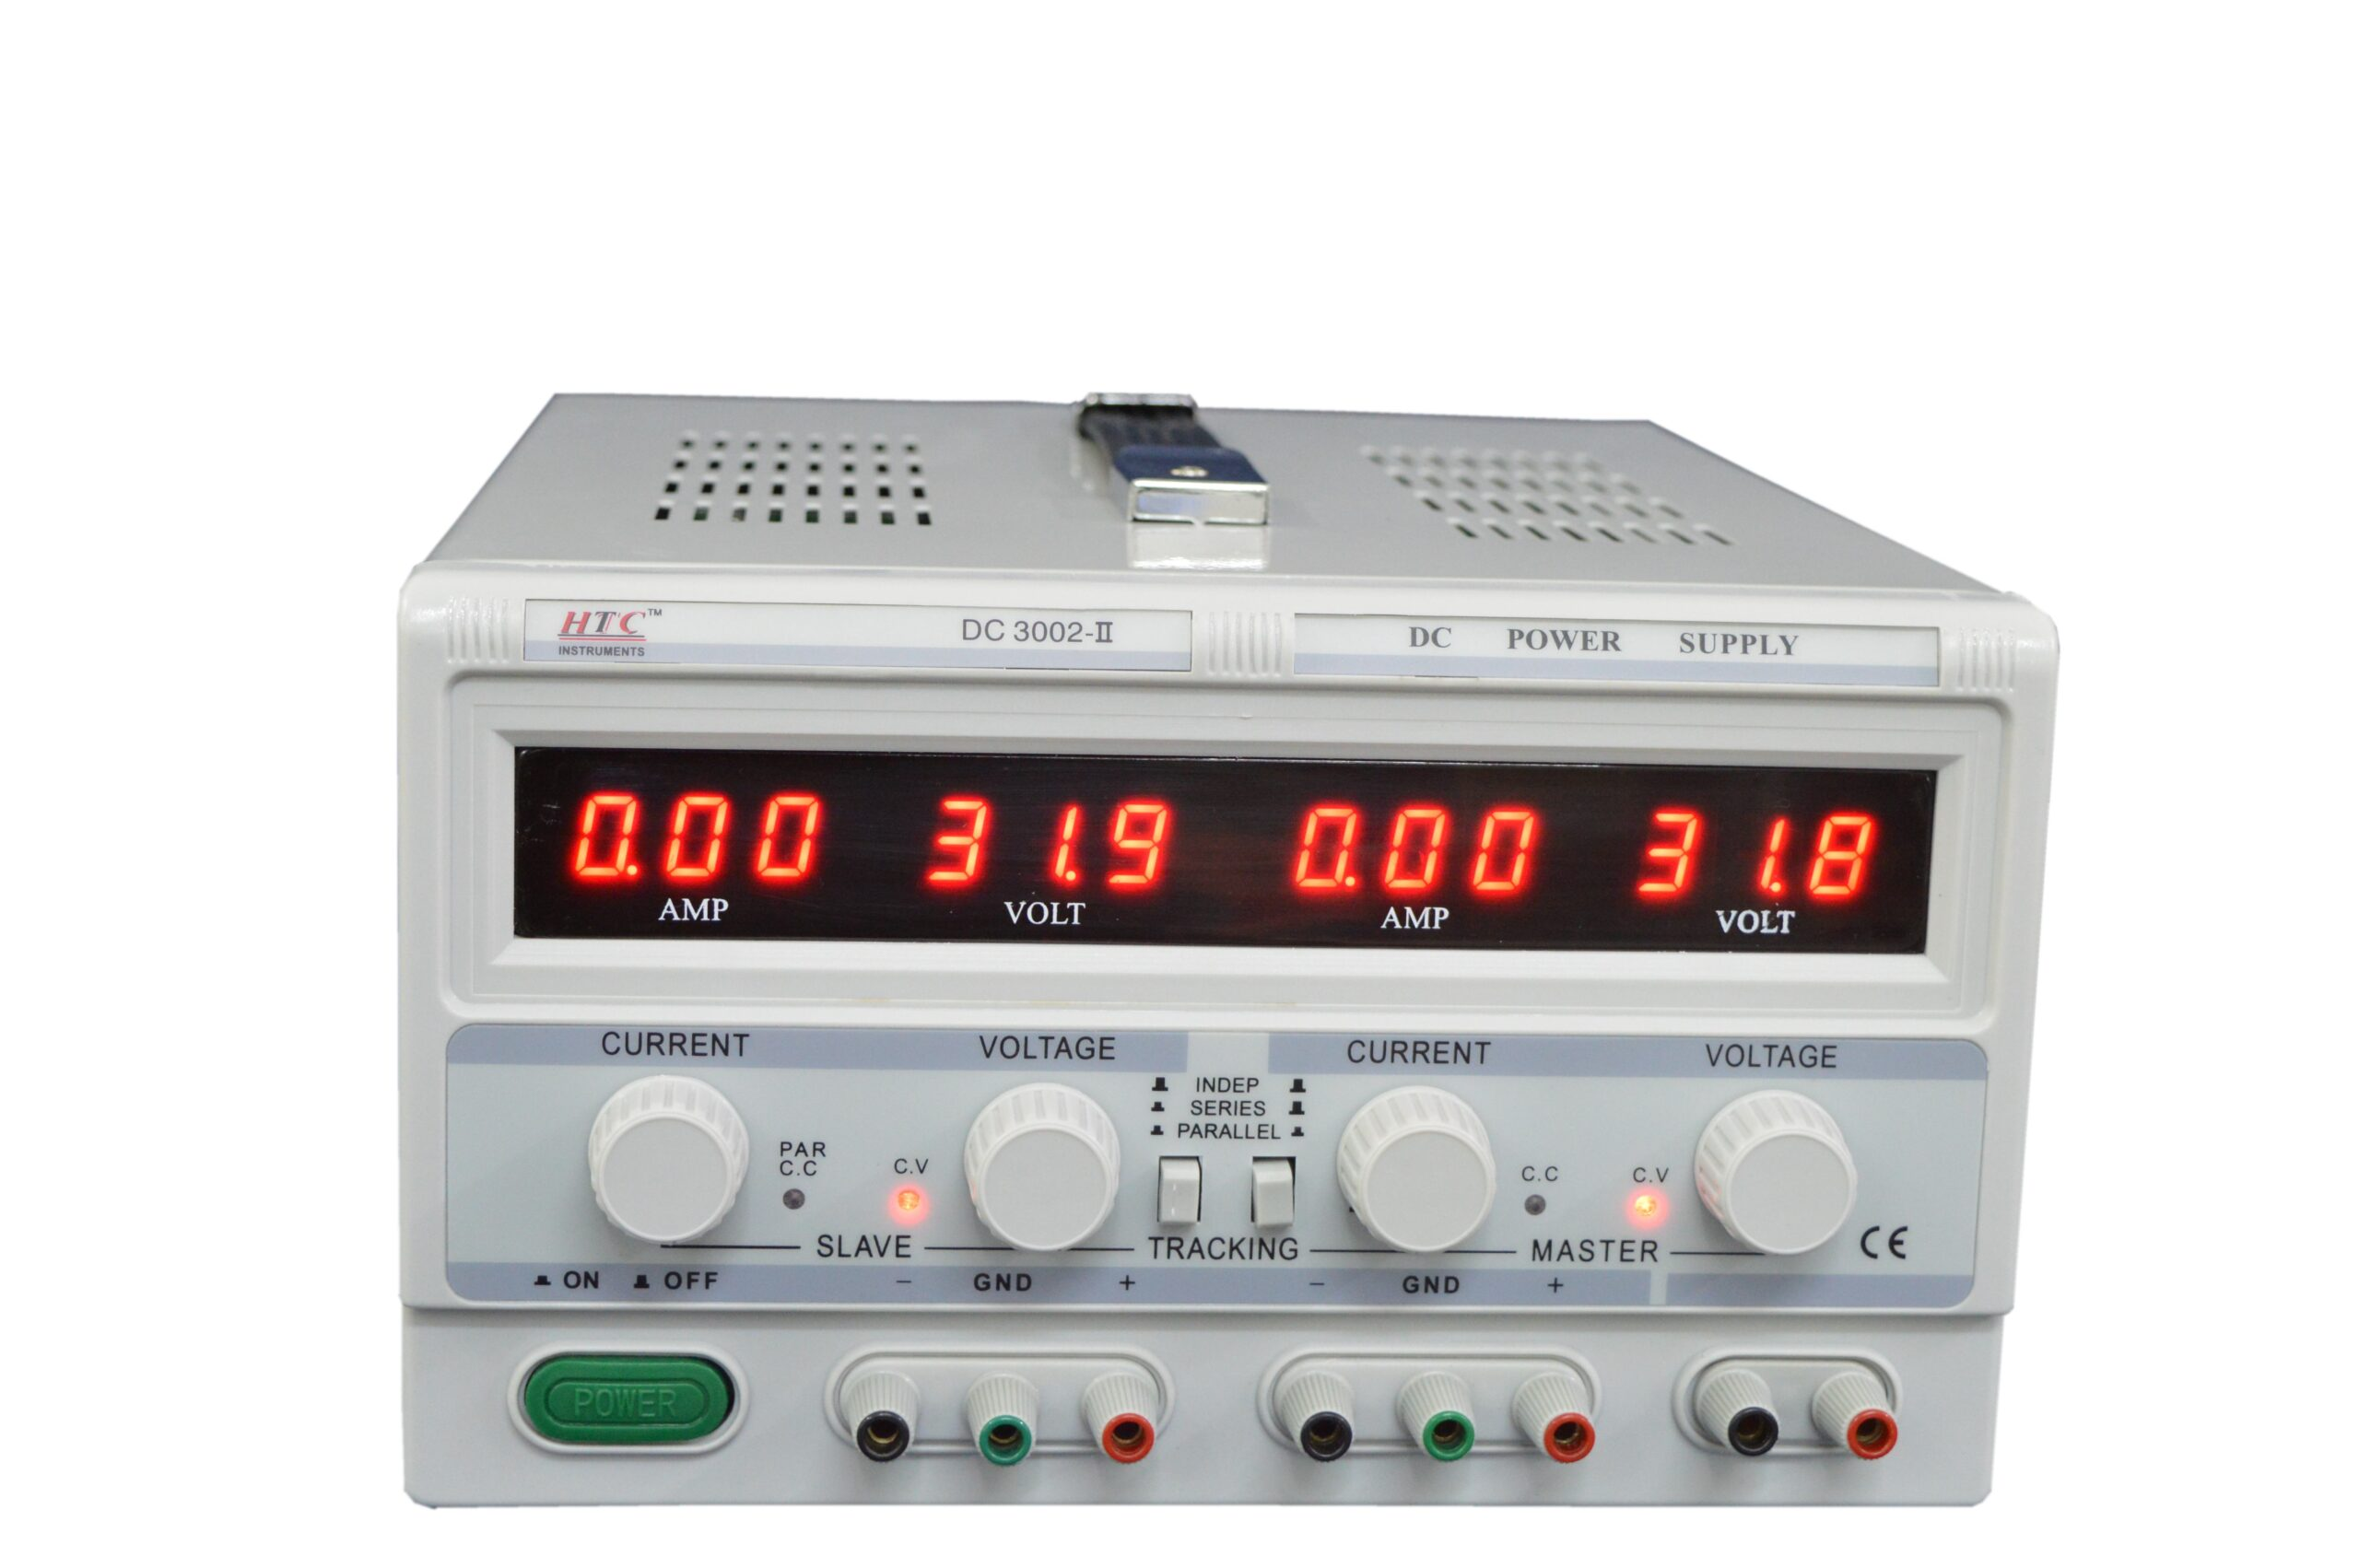
\includegraphics[width=0.5\textwidth]{./images/DC-PowerSupply.jpeg}
					\caption{DC power supply}
					\label{fig:DCPowerSupply}
				\end{figure}

			\subsubsection{Breadboard}
				A breadboard is a construction base for prototyping of electronics.A breadboard consists of plastic block holding a matrix of electrical sockets of a size suitable for gripping thin connecting wire, 
				component wires or the pins of transistors and integrated circuits (ICs). The sockets are connected inside the board, usually in rows of five sockets.

				\begin{figure}[h!]
					\centering
					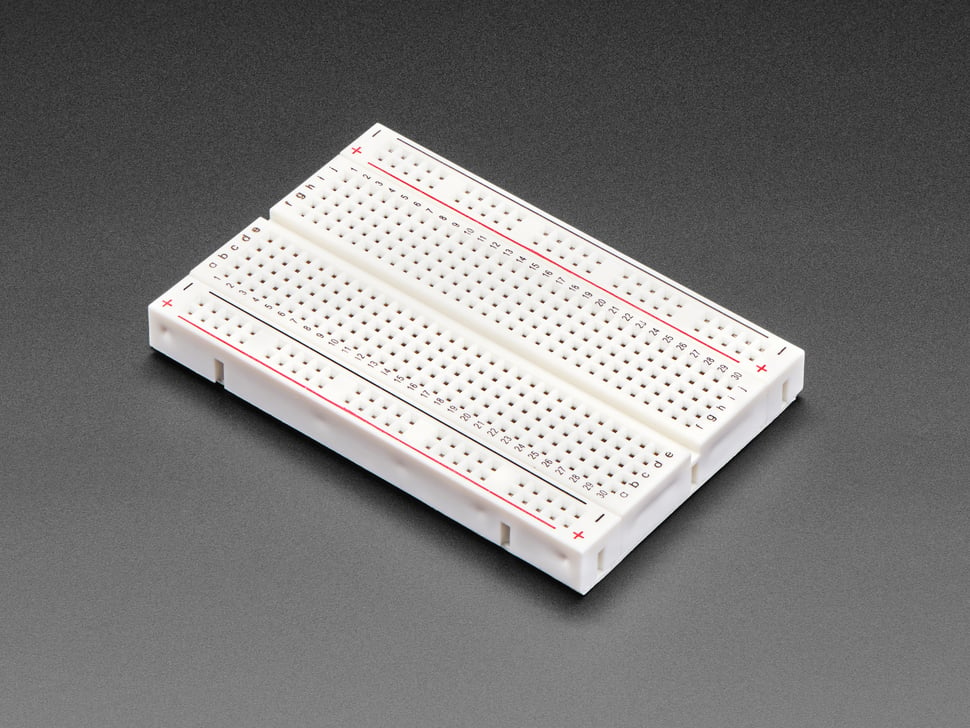
\includegraphics[width=0.5\textwidth]{images/breadboard.jpeg}
					\caption{A breadboard}
					\label{fig:breadboard}
				\end{figure}
			
			\pagebreak
			\subsubsection{Resistors}
				As stated before we needed 3 resistors for this lab report so we took 3 resistors with the proper colour code values and then we measured them and marked them.

				\begin{figure}[h!]
					\centering
					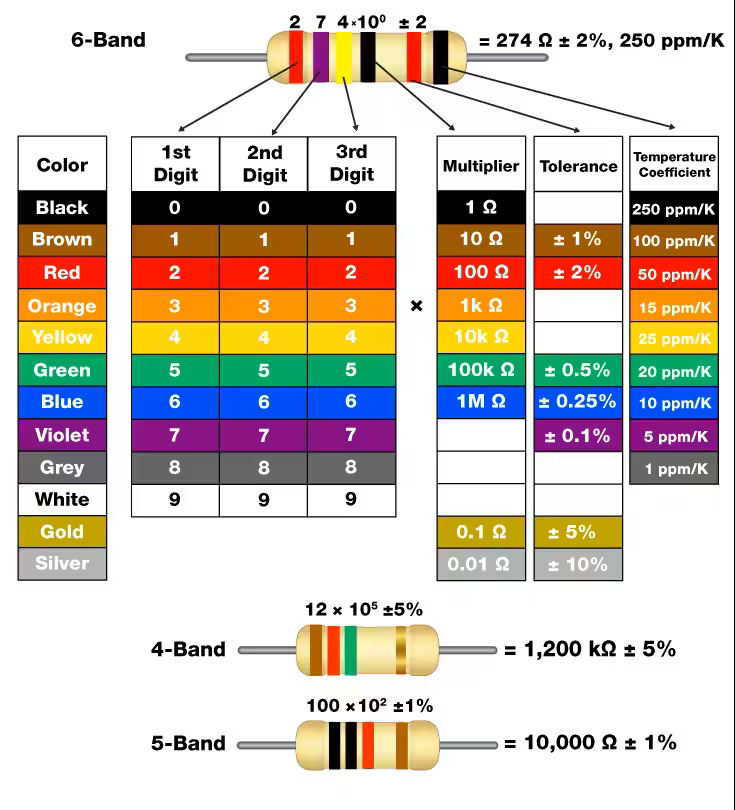
\includegraphics[width=0.35\textwidth]{images/ResistorColorCode.png}
					\caption{Resistors Color Table}
					\label{fig:ResistorsColorTable}
				\end{figure}

	
				\begin{table}[h!]
					\centering
					\begin{tabular}{@{}l|S|S@{}} % l for left, S for siunitx number column
						\toprule
						{Resistor} & {Expected Value (\si{\ohm})} & {Measured Value (\si{\ohm})} \\
						\midrule
						$R_1$ & 1000 & 988 \\
						$R_3$ & 2200 & 2142 \\
						$R_x$ & 2200 & 2169 \\
						\bottomrule
					\end{tabular}
					\caption{Expected and Measured Resistance Values}
					\label{tab:resistors}
				\end{table}

			\pagebreak
			\subsubsection{Multimeter}
				The multimeter is a versatile tool used for measuring various electrical quantities. In this lab, we will use it to measure the voltage drops across components, the currents through branches and components, and the resistance of resistors.
				To measure voltage drops, connect the multimeter in parallel across the component of interest. Set the multimeter to the voltage measurement mode and select an appropriate range.
				To measure currents, connect the multimeter in series with the branch or component. Set the multimeter to the current measurement mode and select an appropriate range.
				To measure resistance, disconnect the resistor from the circuit. Connect the multimeter probes to the resistor terminals. Set the multimeter to the resistance measurement mode and select an appropriate range.

				\begin{figure}[h!]
					\centering
					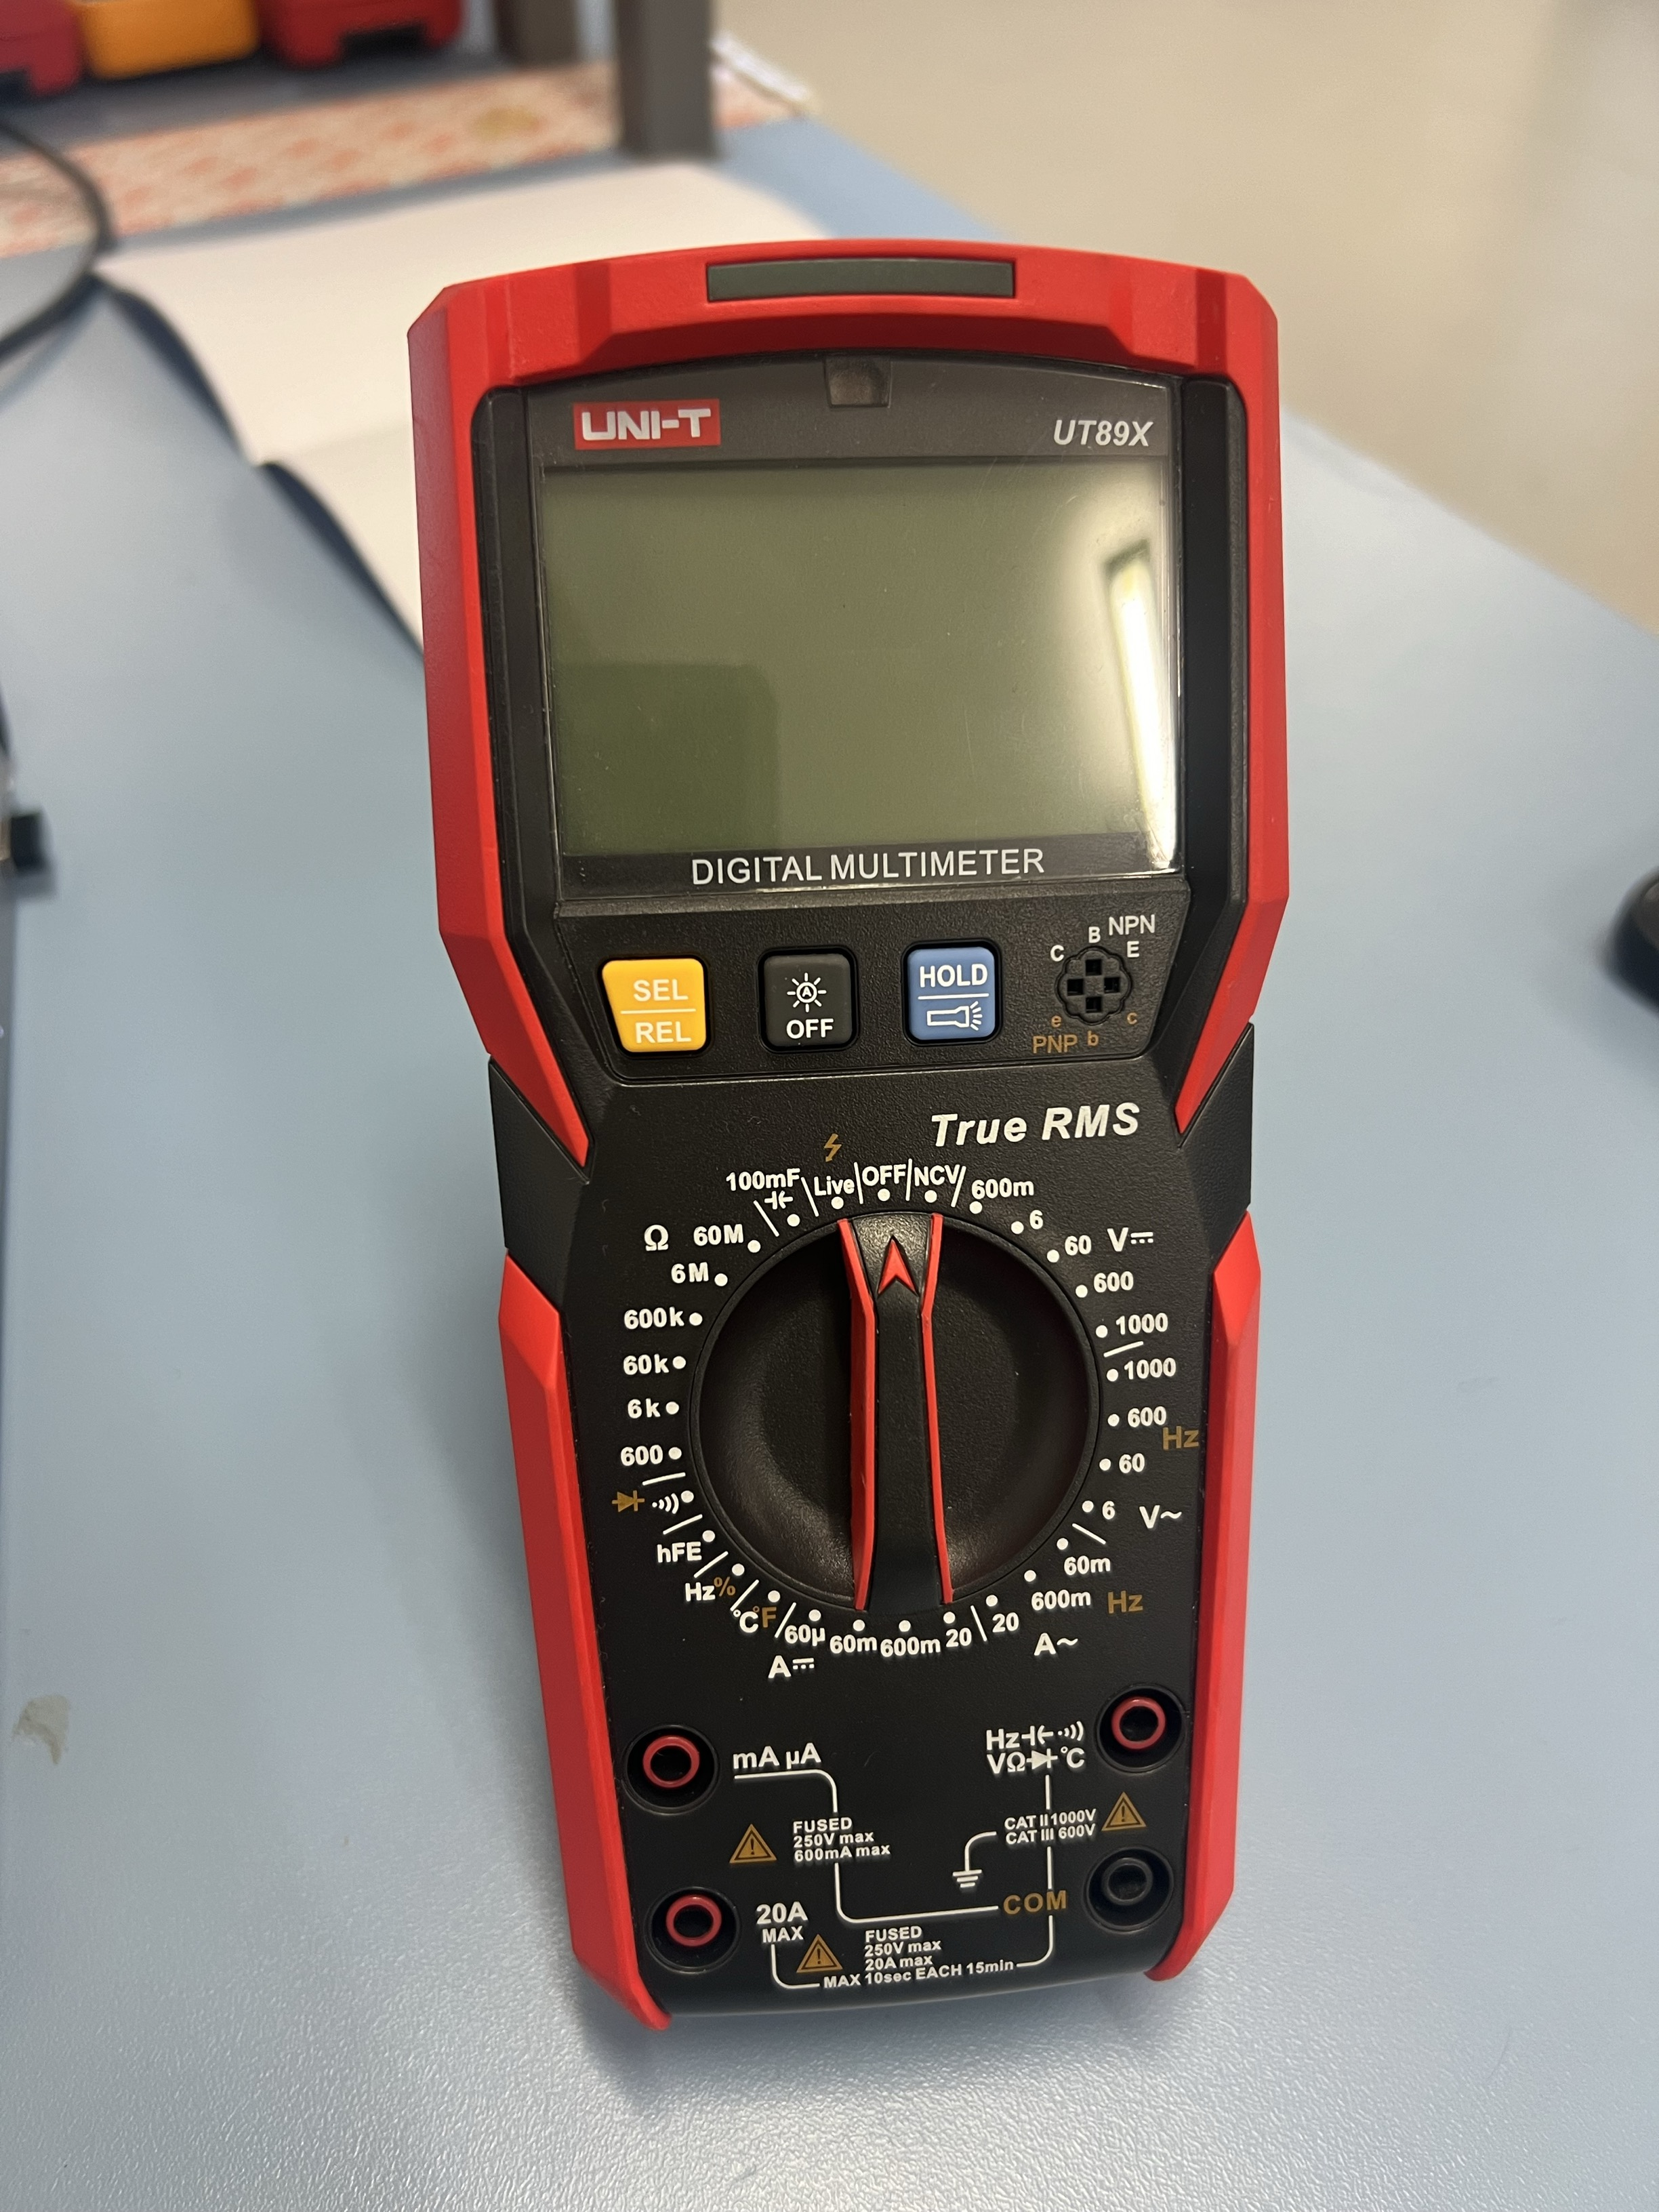
\includegraphics[height = 0.3\textheight]{images/Multimeter.jpeg}
					\caption{Multimeter}
					\label{fig:multi_meter}
				\end{figure}
			
			\subsubsection{Potentiometer}
				A potentiometer is a three-terminal resistor with a sliding ,or rotating, contact that forms an adjustable voltage divider as seen in Figure \ref{fig:potentiometer}.
				If only two terminals are used, one end and the wiper, it acts as a variable resistor.
				\begin{figure}[h!]
					\centering
					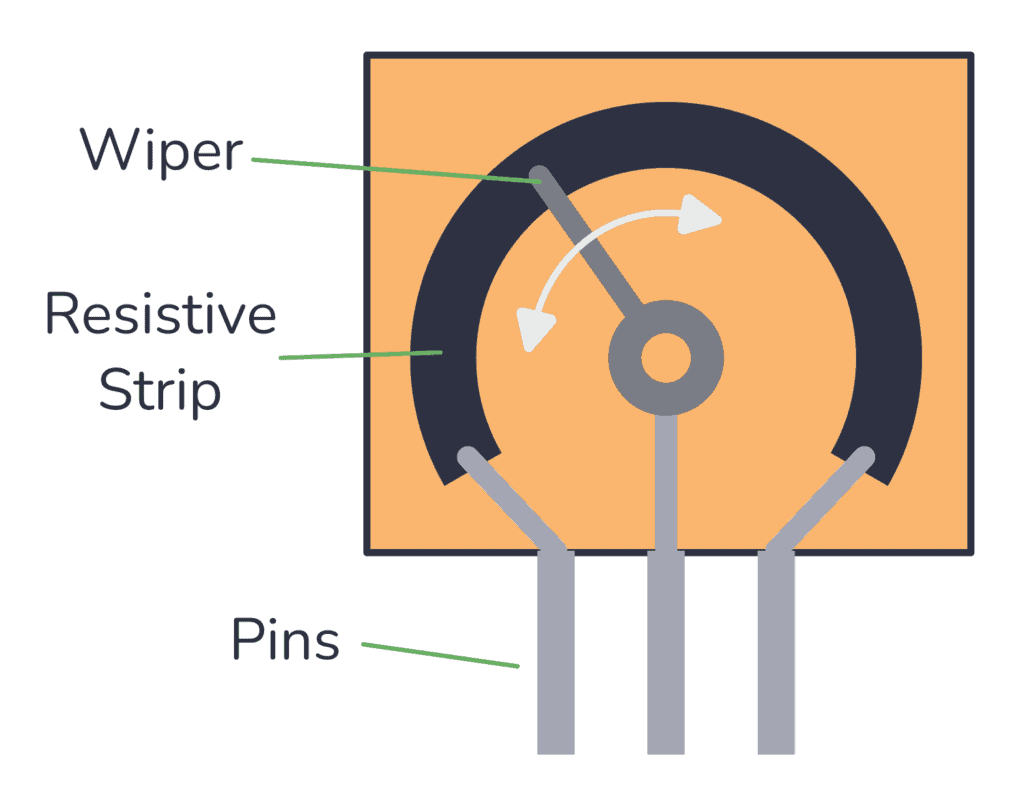
\includegraphics[width=0.5\textwidth]{images/Potentiometer.png}
					\caption{Potentiometer}
					\label{fig:potentiometer}
				\end{figure}
\end{document}
